\documentclass[10pt,a4paper]{amsart}
\usepackage{amsmath,amssymb,amsthm,graphicx}
\usepackage{hyperref}
\usepackage{tikz}
\usetikzlibrary{arrows}

\numberwithin{equation}{section}

\newtheorem{Theorem}{Theorem}[section]
\newtheorem*{Theorem*}{Theorem}
\newtheorem{Corollary}[Theorem]{Corollary}
\newtheorem{Lemma}[Theorem]{Lemma}
\newtheorem{Proposition}[Theorem]{Proposition}
\newtheorem{Conjecture}[Theorem]{Conjecture}

\theoremstyle{definition}
\newtheorem{Definition}[Theorem]{Definition}
\newtheorem{Note}[Theorem]{Note}
\newtheorem{Example}[Theorem]{Example}
\newtheorem{Remark}[Theorem]{Remark}
\usepackage{cleveref}
\crefname{originalreference}{original reference}{original references}
\Crefname{originalreference}{Original reference}{Original references}
\makeatletter
\newlabel{main}{{1.1}{source}{}{sourcepointer-1}{}}
\newlabel{main@cref}{{[originalreference][0][]1.1}{[1][0][]source}{}{}{}}
\makeatother
\title{Realization of arbitrary multiple q-zeta star values as simple graph series}
\author{Antun Milas}
\date{doi:10.3842/SIGMA.2026.087; CC BY 4.0}
\begin{document}
\maketitle
\noindent\textit{Allowed standard prerequisites (editorial).}\begin{itemize}
\item Standard q-binomial summation, vertex-algebra character definitions and classical elliptic/theta functions. Original source bibliography, including Lang, Arakawa and AM where relevant.
\end{itemize}\medskip
\ifdefined\hypertarget\hypertarget{sourcepointer-1}{}\fi
\noindent\textit{Source reference.} Original reference 1.1: algebra-geometry/sources/sigma-2026-087/native/sigma26-087.tex, source lines 202--202. Cross-reference gives an introductory specialization, earlier narrative comparison or section pointer; all source-local arguments used for the counted theorem are included.\par\medskip
Our
approach is motivated on the one hand by our previous work on arc spaces and graph series \cite{BJM,JM1,JM2,HM} (see also \cite{Hao}), and on the other hand by character formulas for certain vertex algebras introduced by Arakawa \cite{Arakawa}, related to genus-zero class-$\mathcal{S}$ theories in physics \cite{BR,Beem}.
As already pointed out in \cite{BJM,JM2,Hao,HM}, the Hilbert series of the arc algebra $J_\infty(R_\Gamma)$, where $R_\Gamma$ is the edge algebra (defined below) of a simple\footnote{It is possible to slightly relax this condition and consider graphs with loops~\cite{Hao}.} graph $\Gamma$, coincides with the character of a certain {\em principal subspace} $W_\Gamma$ (after Feigin and Stoyanovsky~\cite{FS}) inside an appropriate lattice vertex algebra \cite{CLM,Kawasetsu, MP}. Moreover, the arc algebra $J_\infty(R_\Gamma)$ carries the structure of a commutative vertex algebra, and this correspondence can be realized as an isomorphism of commutative graded vertex algebras. We stress, however, that the principal subspace $W_\Gamma$ is not a conformal vertex algebra, so its grading is not canonical.
Therefore, following \cite{Hao}, we equip the principal subspace $W_\Gamma$ with the grading
\[
\deg \bigl({\rm e}^{\alpha_i}_{(-m-1)}\bigr)=m+b_i,
\]
where
\[
Y({\rm e}^{\alpha_i},x)=\sum_{m\in\mathbb{Z}} {\rm e}^{\alpha_i}_{(m)}x^{-m-1},
\]
together with the color grading recording the multiplicity of each generator ${\rm e}^{\alpha_i}$. This grading is the analogue of the grading on the arc algebra $J_\infty(R_\Gamma)$, where the jet variables satisfy
\[
\deg(x_{i,m})=m+b_i.
\]
Thus the correspondence
\[
x_{i,m}
\longleftrightarrow
{\rm e}^{\alpha_i}_{(-m-1)}
\]
preserves both the homogeneous grading and the color grading.

Unless stated otherwise, the variable $q$ records the chosen grading
(conformal in the conformal case and the auxiliary grading described above in
the non-conformal case), while the variables~$x_i$ record the multigrading (or
charge) associated with the generators.

We now return to the connection with arc algebras.
The corresponding Hilbert series of $J_\infty(R_\Gamma)$ is what we call the {\em graph series}
\begin{equation*}%\label{hg}
H_{\Gamma,{\bf b}}(q):=\sum_{{\bf n} \in\mathbb{N}_0^r}
\frac{q^{\frac12 {\bf n}A_\Gamma{\bf n}^{\mathsf{T}}+b_1n_1+\cdots+b_rn_r}}
{(q)_{n_1}\cdots(q)_{n_r}},
\end{equation*}
where $A_\Gamma$ is the (symmetric) adjacency matrix of a graph $\Gamma$ with $r$ vertices and ${\bf b}=(b_1,\dots,b_r)\in\mathbb{N}^r$.
Here we use the standard $q$-Pochhammer notation
\[
(q)_n=\prod_{j=1}^n(1-q^j) \qquad \text{and} \qquad (q)_\infty=\prod_{j=1}^\infty(1-q^j),
\]
 whenever the latter product is viewed formally or converges analytically.
The vector ${\bf b}$ determines the grading of the generators of $W_\Gamma$. Equivalently, we can start from the {\em full} character of~$W_\Gamma$,
\begin{equation*}%\label{hgf}
H_{\Gamma}(q,{\bf x}):=
\sum_{{\bf n}\in\mathbb{N}_0^r}
\frac{{\bf x}^{\bf n}\,
q^{\frac12{\bf n}A_\Gamma{\bf n}^{\mathsf{T}}}}
{(q)_{n_1}\cdots(q)_{n_r}},
\end{equation*}
and specialize to ${\bf x}=q^{\bf b}$. Essentially the same type of $(q,x)$-series appeared in so-called ``knots-quivers'' correspondences; see \cite{Ekholm,Quivers}.

In this paper, we are only interested in the standard grading ${\bf b}=(1,\dots,1)$, in which case
\[
\deg \bigl({\rm e}^{\alpha_i}_{(-m-1)}\bigr)=m+1,
\]
and we simply write $H_\Gamma(q)$ instead of $H_{\Gamma,{\bf b}}(q)$, thus recovering the original graph series introduced in \cite{BJM,JM1,JM2}. Although not directly related to this work, it is worth noting that there is an interesting connection among the Donaldson--Thomas invariants of symmetric quivers, cohomological Hall algebras, and the dual of the principal subspace of $W_{\Gamma}$ \cite{DFR,DM} (see also~\cite{Efimov}).

Since we have encountered a $q$-zeta–type value $\mathfrak{z}_q(k)$, it is natural to ask whether other $q$-multiple zeta values also arise as graph series, possibly with additional Euler factors.
As indicated above, we are primarily interested in the standard grading, corresponding to $b_i = 1$.
Within this framework, the $q$-MZVs relevant to our work were introduced by Ohno, Okuda, and Zudilin in \cite{Ohno}:
\begin{equation} \label{ohno}
\mathfrak{z}_q^*(a_1,\dots,a_k):=\sum_{n_1 \geq n_2 \geq \cdots \geq n_k \geq 1} \frac{q^{n_1}}{(1-q^{n_1})^{a_1} \cdots (1-q^{n_k})^{a_k}}.
\end{equation}
The star symbol indicates that the summation is over non-strict summation variables as opposed to the more standard model:
\[
\mathfrak{z}_q(a_1,\dots,a_k):=\sum_{n_1 > n_2 > \cdots > n_k \geq 1} \frac{q^{n_1}}{(1-q^{n_1})^{a_1} \cdots (1-q^{n_k})^{a_k}}.
\]
The difference between the strict and non-strict $q$-MZV models is controlled by the ``lower depth'' $q$-MZVs, so one can easily transform between the two.
Our next result concerns graph series and multiple $q$-zeta values (\ref{ohno}).

\begin{Theorem} \label{qmzv} For every choice of positive integers $a_1,\dots,a_k$, there is a simple graph $Z_{a_1,\dots,a_k}$ such that
\[
H_{Z_{a_1,\dots,a_k}}(q)=\frac{q^{-1} \mathfrak{z}_q^*(a_1,\dots,a_k)}{(q)^{k+a_1+\cdots +a_k}_\infty}.
\]
In particular, for $k=1$ and $a_1=r$, this recovers $H_{T_{2r+2}}(q)$ and Theorem~{\rm \ref{main}}\,$(ii)$.
\end{Theorem}

\subsection[Graph series and multiple q-zeta series]{Graph series and multiple $\boldsymbol{q}$-zeta series}\label{section2.4}

Now we are ready to explain how to construct all multiple $q$-zeta values in the framework of graph series and thus of vertex algebras. As already discussed in the introduction, we
are interested
in the $q$-MZV model given by
\[
{\mathfrak{z}}_q^*(a_1,\dots,a_k)=\sum_{n_1 \geq n_2 \geq \cdots \geq n_k \geq 1} \frac{q^{n_1}}{(1-q^{n_1})^{a_1} \cdots (1-q^{n_k})^{a_k}}.
\]
Consider a disconnected graph with $2k$ vertices $\{1,\dots,k,1',\dots,k' \}$ and $k$ edges:
\begin{center}
\begin{tikzpicture}[scale=1.2]
% \GraphInit[vstyle=Art]
 % [scale=1.1,auto=left,every node/.style={circle,fill=blue!30}]
 \node (n1) at (1,1) {1};
 \node (n11) at (1.5,1) {1$'$};
 \node (n2) at (2,1) {2};
 \node (n12) at (2.5,1) {2$'$};
 \node (n3) at (3,1) {3};
 \node (n13) at (3.5,1) {3$'$};
 \node (n4) at (4,1) {4};
 \node (n14) at (4.5,1) {4$'$};
 \node (n5) at (5,1) {5};
 \node (n15) at (5.5,1) {5$'$};
 \node (n6) at (6,1) {...};
 \node (n7) at (7,1) {...};
 \node (n8) at (8,1) {...};
 \node (n9) at (9,1) {...};
 \node (n20) at (10.5,1) {$k'$};
 \node (n10) at (10,1) {$k$};

%\path (n8) edge [bend left=30] (n9);
%\path (n8) edge [bend left=40] (n12);
%\path (n1) edge [bend left=20] (n12);
%\path (n3) edge [bend right=20] (n12);
%\path (n11) edge [bend right=40] (n12);
 \foreach \from/\to in {n1/n11,n2/n12,n3/n13,n4/n14,n5/n15,n10/n20}
 \draw (\from) -- (\to);
\end{tikzpicture}
\end{center}
We next construct a graph, denoted by $Z_{a_1,\dots,a_k}$, which will contain the above graph as a subgraph. In this new graph, the nodes denoted by $1',\dots,k'$ are leaves (so they are only adjacent to $1,2,\dots,k$, respectively).

To construct our graph, we attach various simple star graphs to the underlying graph with~$2k$ vertices. For better transparency, in parallel, we consider the graph
$Z_{1,1,1,2,2}$ displayed on Figure~\ref{figure5}.

We first attach $a_1$ simple $(k+1)$-star graphs to the $k$ nodes enumerated by $1,2,\dots,k$ (e.g., on Figure~\ref{figure5}, we attach one $6$-star graph with the central node $6$ to the nodes $1$, $2$, $3$, $4$, $5$).
Then we attach $a_2$ simple star graphs with $k$ legs to the $k-1$ nodes enumerated by $1,2,\dots,k-1$ (e.g., on Figure~\ref{figure5}, we attach one $5$-star graph with central node $8$ to the nodes $1$, $2$, $3$, $4$). We continue until we attach $a_k$ $2$-star graphs (i.e., paths of length two) to node~1 (e.g., on Figure~\ref{figure5}, we attach two $2$-star graphs with central vertices $16$ and $18$ to node~$1$).

\begin{figure}[!ht]\centering
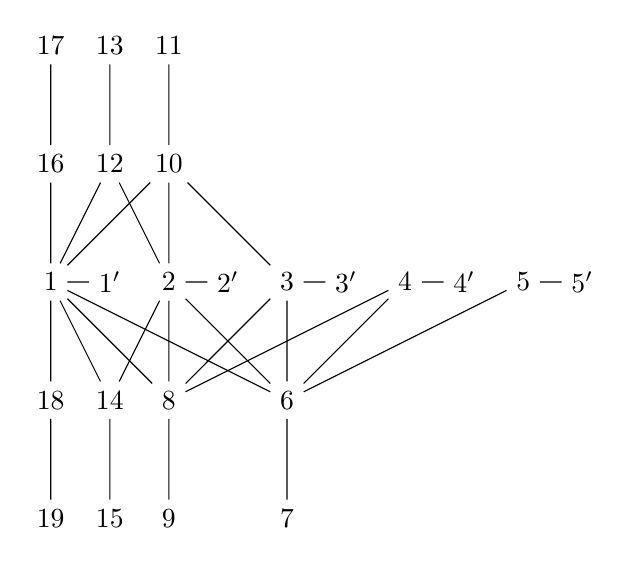
\begin{tikzpicture}[scale=1.5]
% \GraphInit[vstyle=Art]
 % [scale=1.1,auto=left,every node/.style={circle,fill=blue!30}]
 \node (n1) at (1,1) {1};
 \node (n21) at (1.5,1) {1$'$};
 \node (n2) at (2,1) {2};
 \node (n22) at (2.5,1) {2$'$};
 \node (n3) at (3,1) {3};
 \node (n23) at (3.5,1) {3$'$};
 \node (n4) at (4,1) {4};
 \node (n24) at (4.5,1) {4$'$};
 \node (n5) at (5,1) {5};
 \node (n25) at (5.5,1) {5$'$};
 \node (n6) at (3,0) {6};
 \node (n7) at (3,-1) {7};
 \node (n8) at (2,0) {8};
 \node (n9) at (2,-1) {9};
 \node (n10) at (2,2) {10};
 \node (n11) at (2,3) {11};
 \node (n12) at (1.5,2) {12};
 \node (n13) at (1.5,3) {13};
 \node (n14) at (1.5,0) {14};
 \node (n15) at (1.5,-1) {15};
 \node (n16) at (1,2) {16};
 \node (n17) at (1,3) {17};
 \node (n18) at (1,0) {18};
 \node (n19) at (1,-1) {19};

%\path (n8) edge [bend left=30] (n9);
%\path (n8) edge [bend left=40] (n12);
%\path (n1) edge [bend left=20] (n12);
%\path (n3) edge [bend right=20] (n12);
%\path (n11) edge [bend right=40] (n12);
 \foreach \from/\to in {n1/n18,n1/n14,n1/n8,n1/n6,n1/n16,n1/n12,n1/n10,n2/n12,n2/n10,n2/n14,n2/n8,n2/n6,n3/n10,n3/n8,n3/n6,n4/n8,n4/n6,n5/n6,n18/n19,n14/n15,n8/n9,n6/n7,n16/n17,n12/n13,n10/n11,n1/n21,n2/n22,n3/n23,n4/n24,n5/n25}
 \draw (\from) -- (\to);
\end{tikzpicture}
\caption{Graph $Z_{1,1,1,2,2}$.}\label{figure5}
\end{figure}
The Hilbert series of $R_{Z_{a_1, \dots,a_k}}$ can be recursively computed using the relations
\begin{align*}
&H_t(R_{Z_{a_1, \dots,a_k}}) =H_t(R_{Z_{a_1-1, \dots,a_k}})+\frac{t}{(1-t)^{k+1}} \left(\frac{1+t}{1-t}\right)^{a_1+\cdots +a_k-1}, \\
&H_t(R_{Z_{0, \dots,0,a_i,a_{i+1}, \dots, a_k}}) =H_t(R_{Z_{a_i, \dots,a_k}}).
\end{align*}
A closed formula for $H_t(R_{Z_{a_1, \dots,a_k}})$ is somewhat messy so we do not display it here.

For the graph series, we have the following result:
\[
H_{Z_{a_1,\dots,a_k}}(q)=\frac{q^{-1}{\mathfrak{z}}^*_q(a_1,\dots,a_k)}{(q)_\infty^{a_1+\cdots +a_k+k}}.
\]
\begin{proof}[Proof of Theorem~\ref{qmzv}]
Again, the proof is easier to follow by considering an example in~parallel; see Figure~\ref{figure5}.
We first sum over all $(k+1)$-star subgraphs. By definition, there are $a_1$ such subgraphs.
For each subgraph, we start from the leaf node $s$ (for instance, node 7 in Figure~\ref{figure5}) and the central node $t$ (for instance, node 6 in Figure~\ref{figure5}).
This leads to the following summation:
\begin{align*}
\sum_{n_s,n_t \geq 0} \frac{q^{n_s(n_t+1)+n_t(n_1+\cdots + n_k+1)}}{(q)_{n_s}(q)_{n_t}}
=\sum_{n_t \geq 0} \frac{q^{n_t(n_1+\cdots + n_k+1)}}{(q^{n_t+1})_\infty (q)_{n_t} }= \frac{1}{(q)_\infty \bigl(1-q^{n_1+\cdots +n_k+1}\bigr)}.
\end{align*}
Repeating this $a_1$ times (observe that the summation variables corresponding to the relevant subgraphs are independent) results with
\[
\frac{1}{(q)^{a_1}_\infty \bigl(1-q^{n_1+\cdots +n_k+1}\bigr)^{a_1}}.
\]
We repeat the same procedure for $k$-star graphs attached to $1,2,\dots,k-1$. These subgraphs contribute with
\[
\frac{1}{(q)^{a_2}_\infty \bigl(1-q^{n_1+\cdots +n_{k-1}+1}\bigr)^{a_2}}.
\]
We continue until we sum over paths of length two (e.g., nodes 17 and 16) attached to the node $1$. Here the contribution is
\[
\frac{1}{(q)^{a_k}_\infty \bigl(1-q^{n_1+1}\bigl)^{a_k}}.
\]
We also have to sum over the variables that correspond to the ``prime'' nodes:
\[
\sum_{ n_1',\dots,n_k' \geq 0} \frac{q^{n_1'(n_1+1)+\cdots + n_k'(n_k+1)}}{(q)_{n_1'} \cdots (q)_{n_k'}}=\frac{1}{\bigl(q^{n_1+1}\bigr)_\infty \cdots \bigl(q^{n_k+1}\bigr)_\infty}.
\]
Combining everything with the final $k$-fold summation over $n_1,\dots,n_k$, we quickly get
\[
\frac{1}{(q)_\infty^{\sum_{i=1}^k a_i+k}} \sum_{n_1,\dots,n_k \geq 0} \frac{q^{n_1+ \cdots + n_k}}{\bigl(1-q^{\sum_{i=1}^{k} n_i+1}\bigr)^{a_1} \bigl(1-q^{\sum_{i=1}^{k-1} n_i+1}\bigr)^{a_2} \cdots \bigl(1-q^{n_1+1}\bigr)^{a_k}}.
\]
Setting $n_1+n_2+\cdots + n_k+1 \to m_1$, $n_1+n_2+\cdots + n_k+1 \to m_2,\dots,n_1+1 \to m_k$ proves the claim.
\end{proof}

\begin{thebibliography}{99}
\footnotesize\itemsep=0pt

\bibitem{AM}
Adamovi\'{c} D., Milas A., On some vertex algebras related to
 {$V_{-1}(\mathfrak{sl}(n))$} and their characters,
 \href{https://doi.org/10.1007/s00031-020-09617-w}{\textit{Transform. Groups}}
 \textbf{26} (2021), 1--30,
 \href{https://arxiv.org/abs/1805.09771}{arXiv:1805.09771}.

\bibitem{Andrews0}
Andrews G.E., The theory of partitions, \textit{Encyclopedia Math. Appl.},
 Vol.~2, Addison-Wesley Publishing Co., Reading, Mass., 1976.

\bibitem{Andrews}
Andrews G.E., Stacked lattice boxes,
 \href{https://doi.org/10.1007/BF01608779}{\textit{Ann. Comb.}} \textbf{3}
 (1999), 115--130.

\bibitem{AR}
Andrews G.E., Rose S.C.F., Mac{M}ahon's sum-of-divisors functions, {C}hebyshev
 polynomials, and quasi-modular forms,
 \href{https://doi.org/10.1515/crelle.2011.179}{\textit{J.~Reine Angew.
 Math.}} \textbf{676} (2013), 97--103,
 \href{https://arxiv.org/abs/1010.5769}{arXiv:1010.5769}.

\bibitem{Arakawa}
Arakawa T., Chiral algebras of class $\mathcal{S}$ and {M}oore--{T}achikawa
 symplectic varieties,
 \href{https://arxiv.org/abs/1811.01577}{arXiv:1811.01577}.

\bibitem{AK}
Arakawa T., Kawasetsu K., Quasi-lisse vertex algebras and modular linear
 differential equations, in Lie Groups, Geometry, and Representation Theory,
 \textit{Progr. Math.}, Vol. 326,
 \href{https://doi.org/10.1007/978-3-030-02191-7_2}{Birkh\"auser}, Cham, 2018,
 41--57, \href{https://arxiv.org/abs/1610.05865}{arXiv:1610.05865}.

\bibitem{BK2}
Bachmann H., K\"uhn U., A short note on a conjecture of {O}kounkov about a
 $q$-analogue of multiple zeta values,
 \href{https://arxiv.org/abs/1407.6796}{arXiv:1407.6796}.

\bibitem{BK1}
Bachmann H., K\"uhn U., The algebra of generating functions for multiple
 divisor sums and applications to multiple zeta values,
 \href{https://doi.org/10.1007/s11139-015-9707-7}{\textit{Ramanujan~J.}}
 \textbf{40} (2016), 605--648,
 \href{https://arxiv.org/abs/1309.3920}{arXiv:1309.3920}.

\bibitem{BK3}
Bachmann H., K\"uhn U., A dimension conjecture for $q$-analogues of multiple
 zeta values, in Periods in Quantum Field Theory and Arithmetic,
 \textit{Springer Proc. Math. Stat.}, Vol.~314,
 \href{https://doi.org/10.1007/978-3-030-37031-2_9}{Springer}, Cham, 2020,
 237--258, \href{https://arxiv.org/abs/1708.07464}{arXiv:1708.07464}.

\bibitem{BR}
Beem C., Lemos M., Liendo P., Peelaers W., Rastelli L., van Rees B.C., Infinite
 chiral symmetry in four dimensions,
 \href{https://doi.org/10.1007/s00220-014-2272-x}{\textit{Comm. Math. Phys.}}
 \textbf{336} (2015), 1359--1433,
 \href{https://arxiv.org/abs/1312.5344}{arXiv:1312.5344}.

\bibitem{Beem}
Beem C., Rastelli L., Vertex operator algebras, {H}iggs branches, and modular
 differential equations,
 \href{https://doi.org/10.1007/jhep08(2018)114}{\textit{J.~High Energy Phys.}}
 \textbf{2018} (2018), no.~8, 114, 72~pages,
 \href{https://arxiv.org/abs/1707.07679}{arXiv:1707.07679}.

\bibitem{Beem-new}
Beem C., Singh P., Razamat S.S., Schur indices of class {$\mathcal{S}$} and
 quasimodular forms,
 \href{https://doi.org/10.1103/physrevd.105.085009}{\textit{Phys. Rev.~D}}
 \textbf{105} (2022), 085009, 15~pages,
 \href{https://arxiv.org/abs/2112.10715}{arXiv:2112.10715}.

\bibitem{Bradley}
Bradley D.M., Multiple {$q$}-zeta values,
 \href{https://doi.org/10.1016/j.jalgebra.2004.09.017}{\textit{J.~Algebra}}
 \textbf{283} (2005), 752--798,
 \href{https://arxiv.org/abs/math/0402093}{arXiv:math/0402093}.

\bibitem{BFM}
Bringmann K., Folsom A., Mahlburg K., Quasimodular forms and
 {$s\ell(m|m)^\wedge$} characters,
 \href{https://doi.org/10.1007/s11139-014-9621-4}{\textit{Ramanujan~J.}}
 \textbf{36} (2015), 103--116,
 \href{https://arxiv.org/abs/1302.4040}{arXiv:1302.4040}.

\bibitem{BJM}
Bringmann K., Jennings-Shaffer C., Milas A., Graph schemes, graph series, and
 modularity,
 \href{https://doi.org/10.1016/j.jcta.2023.105749}{\textit{J.~Combin. Theory
 Ser.~A}} \textbf{197} (2023), 105749, 37~pages,
 \href{https://arxiv.org/abs/2105.05660}{arXiv:2105.05660}.

\bibitem{BVM}
Bringmann K., Milas A., van Ittersum J.W.M., Quasimodularity  of $q$-series associated to root lattices, {i}n preparation.

\bibitem{CLM}
Calinescu C., Lepowsky J., Milas A., Vertex-algebraic structure of the
 principal subspaces of level one modules for the untwisted affine {L}ie
 algebras of types {$A$, $D$, $E$},
 \href{https://doi.org/10.1016/j.jalgebra.2009.09.029}{\textit{J.~Algebra}}
 \textbf{323} (2010), 167--192,
 \href{https://arxiv.org/abs/0908.4054}{arXiv:0908.4054}.

\bibitem{Carlsson}
Carlsson E., Vertex operators, {G}rassmannians, and {H}ilbert schemes,
 \href{https://doi.org/10.1007/s00220-010-1123-7}{\textit{Comm. Math. Phys.}}
 \textbf{300} (2010), 599--613,
 \href{https://arxiv.org/abs/0910.5528}{arXiv:0910.5528}.

\bibitem{DMN}
Dong C., Mason G., Nagatomo K., Quasi-modular forms and trace functions
 associated to free boson and lattice vertex operator algebras,
 \href{https://doi.org/10.1155/S1073792801000204}{\textit{Int. Math. Res.
 Not.}} \textbf{2001} (2001), 409--427,
 \href{https://arxiv.org/abs/math/0004132}{arXiv:math/0004132}.

\bibitem{DFR}
Dotsenko V., Feigin E., Reineke M., Koszul algebras and {D}onaldson--{T}homas
 invariants, \href{https://doi.org/10.1007/s11005-022-01604-4}{\textit{Lett.
 Math. Phys.}} \textbf{112} (2022), 106, 39~pages,
 \href{https://arxiv.org/abs/2111.07588}{arXiv:2111.07588}.

\bibitem{DM}
Dotsenko V., Mozgovoy S., D{T} invariants from vertex algebras,
 \href{https://doi.org/10.1017/S1474748024000288}{\textit{J.~Inst. Math.
 Jussieu}} \textbf{24} (2025), 291--339,
 \href{https://arxiv.org/abs/2108.10338}{arXiv:2108.10338}.

\bibitem{Efimov}
Efimov A.I., Cohomological {H}all algebra of a symmetric quiver,
 \href{https://doi.org/10.1112/S0010437X12000152}{\textit{Compos. Math.}}
 \textbf{148} (2012), 1133--1146,
 \href{https://arxiv.org/abs/1103.2736}{arXiv:1103.2736}.

\bibitem{Ekholm}
Ekholm T., Gruen A., Gukov S., Kucharski P., Park S., Sto\v{s}i\'{c} M.,
 Su{\l}kowski P., Branches, quivers, and ideals for knot complements,
 \href{https://doi.org/10.1016/j.geomphys.2022.104520}{\textit{J.~Geom.
 Phys.}} \textbf{177} (2022), 104520, 75~pages,
 \href{https://arxiv.org/abs/2110.13768}{arXiv:2110.13768}.

\bibitem{FS}
Feigin B., Stoyanovsky A.V., Quasi-particles models for the representations of
 {L}ie algebras and geometry of flag manifold,
 \href{https://arxiv.org/abs/hep-th/9308079}{arXiv:hep-th/9308079}.

\bibitem{Goncharov}
Goncharov A.B., Multiple polylogarithms, cyclotomy and modular complexes,
 \href{https://doi.org/10.4310/MRL.1998.v5.n4.a7}{\textit{Math. Res. Lett.}}
 \textbf{5} (1998), 497--516.

\bibitem{GM}
Goujard E., M\"{o}ller M., Counting {F}eynman-like graphs: {Q}uasimodularity
 and {S}iegel--{V}eech weight,
 \href{https://doi.org/10.4171/jems/924}{\textit{J.~Eur. Math. Soc. (JEMS)}}
 \textbf{22} (2020), 365--412,
 \href{https://arxiv.org/abs/1609.01658}{arXiv:1609.01658}.

\bibitem{CM}
Herzog J., Hibi T., Distributive lattices, bipartite graphs and {A}lexander
 duality,
 \href{https://doi.org/10.1007/s10801-005-4528-1}{\textit{J.~Algebraic
 Combin.}} \textbf{22} (2005), 289--302,
 \href{https://arxiv.org/abs/math/0307235}{arXiv:math/0307235}.

\bibitem{Hoffman}
Hoffman M.E., Algebraic aspects of multiple zeta values, in Zeta Functions,
 Topology and Quantum Physics, \textit{Dev. Math.}, Vol.~14,
 \href{https://doi.org/10.1007/0-387-24981-8_4}{Springer}, New York, 2005,
 51--73, \href{https://arxiv.org/abs/math/0309425}{arXiv:math/0309425}.

\bibitem{Zagier1}
Ihara K., Kaneko M., Zagier D., Derivation and double shuffle relations for
 multiple zeta values,
 \href{https://doi.org/10.1112/S0010437X0500182X}{\textit{Compos. Math.}}
 \textbf{142} (2006), 307--338.

\bibitem{JM1}
Jennings-Shaffer C., Milas A., On {$q$}-series identities for false theta
 series, \href{https://doi.org/10.1016/j.aim.2020.107411}{\textit{Adv. Math.}}
 \textbf{375} (2020), 107411, 22~pages,
 \href{https://arxiv.org/abs/2001.11368}{arXiv:2001.11368}.

\bibitem{JM2}
Jennings-Shaffer C., Milas A., Further {$q$}-series identities and conjectures
 relating false theta functions and characters, in Lie groups, Number Theory,
 and Vertex Algebras, \textit{Contemp. Math.}, Vol.~768,
 \href{https://doi.org/10.1090/conm/768/15467}{American Mathematical Society},
 Providence, RI, 2021, 253--269,
 \href{https://arxiv.org/abs/2005.13620}{arXiv:2005.13620}.

\bibitem{Kawasetsu}
Kawasetsu K., The free generalized vertex algebras and generalized principal
 subspaces,
 \href{https://doi.org/10.1016/j.jalgebra.2015.07.014}{\textit{J.~Algebra}}
 \textbf{444} (2015), 20--51,
 \href{https://arxiv.org/abs/1502.05276}{arXiv:1502.05276}.

\bibitem{Quivers}
Kucharski P., Reineke M., Sto\v{s}i\'{c} M., Su{\l}kowski P., Knots-quivers
 correspondence,
 \href{https://doi.org/10.4310/atmp.2019.v23.n7.a4}{\textit{Adv. Theor. Math.
 Phys.}} \textbf{23} (2019), 1849--1902,
 \href{https://arxiv.org/abs/1707.04017}{arXiv:1707.04017}.

\bibitem{Lang}
Lang S., Elliptic functions, 2nd ed., \textit{Grad. Texts in Math.}, Vol.~112,
 \href{https://doi.org/10.1007/978-1-4612-4752-4}{Springer}, New York, 1987.

\bibitem{Hao}
Li H., Some remarks on associated varieties of vertex operator superalgebras,
 \href{https://doi.org/10.1007/s40879-021-00477-6}{\textit{Eur.~J. Math.}}
 \textbf{7} (2021), 1689--1728,
 \href{https://arxiv.org/abs/2007.04522}{arXiv:2007.04522}.

\bibitem{HM}
Li H., Milas A., Jet schemes, quantum dilogarithm and {F}eigin--{S}toyanovsky's
 principal subspaces,
 \href{https://doi.org/10.1016/j.jalgebra.2023.10.033}{\textit{J.~Algebra}}
 \textbf{640} (2024), 21--58,
 \href{https://arxiv.org/abs/2010.02143}{arXiv:2010.02143}.

\bibitem{Libgober}
Libgober A., Elliptic genera, real algebraic varieties and quasi-{J}acobi
 forms, in Topology of Stratified Spaces, \textit{Math. Sci. Res. Inst.
 Publ.}, Vol.~58, Cambridge University Press, Cambridge, 2011, 95--120,
 \href{https://arxiv.org/abs/0904.1026}{arXiv:0904.1026}.

\bibitem{M2}
Milas A., Formal differential operators, vertex operator algebras and
 zeta-values,~{II},
 \href{https://doi.org/10.1016/S0022-4049(03)00036-7}{\textit{J.~Pure Appl.
 Algebra}} \textbf{183} (2003), 191--244,
 \href{https://arxiv.org/abs/math/0303154}{arXiv:math/0303154}.

\bibitem{M1}
Milas A., On certain automorphic forms associated to rational vertex operator
 algebras, in Moonshine: The First Quarter Century and Beyond, \textit{London
 Math. Soc. Lecture Note Ser.}, Vol.~372,
 \href{https://doi.org/10.1017/CBO9780511730054.016}{Cambridge University
 Press}, Cambridge, 2010, 330--357.

\bibitem{MP}
Milas A., Penn M., Lattice vertex algebras and combinatorial bases: general
 case and {$\mathcal W$}-algebras, \textit{New York J. Math.} \textbf{18}
 (2012), 621--650.

\bibitem{Ob-Serre}
Oberdieck G., A {S}erre derivative for even weight {J}acobi forms,
 \href{https://arxiv.org/abs/1209.5628}{arXiv:1209.5628}.

\bibitem{Ob}
Oberdieck G., Gromov--{W}itten invariants of the {H}ilbert schemes of points of
 a {K}3 surface, \href{https://doi.org/10.2140/gt.2018.22.323}{\textit{Geom.
 Topol.}} \textbf{22} (2018), 323--437,
 \href{https://arxiv.org/abs/1406.1139}{arXiv:1406.1139}.

\bibitem{Ohno}
Ohno Y., Okuda J., Zudilin W., Cyclic {$q$}-{MZSV} sum,
 \href{https://doi.org/10.1016/j.jnt.2011.08.001}{\textit{J.~Number Theory}}
 \textbf{132} (2012), 144--155.

\bibitem{Zagier2}
Ohno Y., Zagier D., Multiple zeta values of fixed weight, depth, and height,
 \href{https://doi.org/10.1016/S0019-3577(01)80037-9}{\textit{Indag.
 Math.~(N.S.)}} \textbf{12} (2001), 483--487.

\bibitem{Okounkov}
Okunkov A., Hilbert schemes and multiple {$q$}-zeta values,
 \href{https://doi.org/10.1007/s10688-014-0054-z}{\textit{Funct. Anal. Appl.}}
 \textbf{48} (2014), 138--144,
 \href{https://arxiv.org/abs/1404.3873}{arXiv:1404.3873}.

\bibitem{OEIS}
The on-line encyclopedia of integer sequences, \url{https://oeis.org/}.

\bibitem{Pan}
Pan Y., Peelaers W., Exact {S}chur index in closed form,
 \href{https://doi.org/10.1103/physrevd.106.045017}{\textit{Phys. Rev.~D}}
 \textbf{106} (2022), 045017, 34~pages,
 \href{https://arxiv.org/abs/2112.09705}{arXiv:2112.09705}.

\bibitem{Qin}
Qin Z., Yu F., On {O}kounkov's conjecture connecting {H}ilbert schemes of
 points and multiple {$q$}-zeta values,
 \href{https://doi.org/10.1093/imrn/rnw244}{\textit{Int. Math. Res. Not.}}
 \textbf{2018} (2018), 321--361,
 \href{https://arxiv.org/abs/1510.00837}{arXiv:1510.00837}.

\bibitem{Edge}
Renteln P., The {H}ilbert series of the face ring of a flag complex,
 \href{https://doi.org/10.1007/s003730200045}{\textit{Graphs Combin.}}
 \textbf{18} (2002), 605--619.

\bibitem{Ittersum}
van Ittersum J.W.M., Partitions and quasimodular forms: {V}ariations on the
 {B}loch--{O}kounkov theorem, Ph.D. thesis, {U}trecht {U}niversity, 2021,
 \url{https://staff.fnwi.uva.nl/j.w.m.vanittersum/files/theses/thesis_vanIttersum_withcover.pdf}.

\bibitem{Zagier}
Zagier D., Multiple zeta values, {P}reprint, 1995.

\bibitem{Zhu}
Zhu Y., Modular invariance of characters of vertex operator algebras,
 \href{https://doi.org/10.1090/S0894-0347-96-00182-8}{\textit{J.~Amer. Math.
 Soc.}} \textbf{9} (1996), 237--302.

\bibitem{Zudilin2}
Zudilin W., Algebraic relations for multiple zeta values,
 \href{https://doi.org/10.1070/RM2003v058n01ABEH000592}{\textit{Russian Math.
 Surveys}} \textbf{58} (2003), 1--29.

\bibitem{Zudilin1}
Zudilin W., Multiple $q$-zeta brackets,
 \href{https://doi.org/10.3390/math3010119}{\textit{Mathematics}} \textbf{3}
 (2015), 119--130, \href{https://arxiv.org/abs/1412.0163}{arXiv:1412.0163}.

\end{thebibliography}
\end{document}
